\chapter[建模]{第 1 讲\quad 建模：把一台机器写成方程}
\label{ch:model}

\begin{quote}\small
\textbf{本讲目标}\quad 从零推导出小车倒立摆的运动方程，理解三件事：
为什么它难（欠驱动、非线性、不稳定）、
为什么它可解（小车通道恒可逆）、
以及后面每一讲都要反复用到的两个工具——能量与线性化。\\[2pt]
\textbf{前置}\quad 拉格朗日力学（会用即可）、矩阵、常微分方程。\\
\textbf{视频}\quad 约 4 分钟（成片 3:43）。\quad\textbf{代码}\quad \texttt{build/plant.py}。
\end{quote}

\section{为什么从这一台小车开始}

控制课的例子很多，但很少有系统能同时具备下面四条性质：

\begin{enumerate}[leftmargin=2em,itemsep=3pt]
  \item \textbf{欠驱动}：两个自由度（小车位置 $p$、摆杆角度 $\theta$），只有一个输入（作用在小车上的力 $u$）。
        你无法直接"命令"摆杆怎么转。
  \item \textbf{本质非线性}：方程里出现 $\sin\theta$、$\cos\theta$、$\dot\theta^2$ 的乘积，
        线性近似只在十几度的范围内有效。
  \item \textbf{开环不稳定}：直立平衡点的线性化有一个正实特征值，
        微小偏差会以 $0.25$\,s 的时间常数指数放大。
  \item \textbf{可实验}：它便宜、安全、能 50\,Hz 实时跑，适合把所有结论都验证一遍。
\end{enumerate}

前三条决定了它"不好控"，第四条决定了它"适合教学"。后面的十讲会反复出现一个模式：
\textbf{先看一个方法在哪里失效，再去理解为什么需要下一个方法}。

\section{系统、坐标与假设}

\begin{figure}[htbp]
\centering
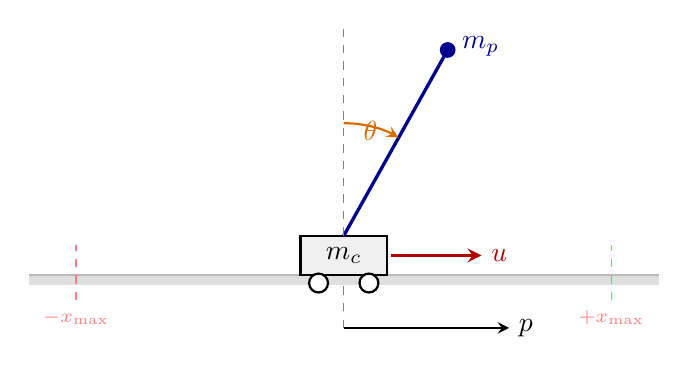
\begin{tikzpicture}[>=stealth,scale=1.0]
  % rail
  \fill[gray!25] (-4,0) rectangle (4,0.12);
  \draw[gray!55,thick] (-4,0.12) -- (4,0.12);
  % cart
  \draw[fill=gray!12,thick] (-0.55,0.12) rectangle (0.55,0.62);
  \node at (0,0.37) {$m_c$};
  % wheels
  \draw[fill=white,thick] (-0.32,0.02) circle (0.12);
  \draw[fill=white,thick] (0.32,0.02) circle (0.12);
  % pole
  \draw[very thick,blue!55!black] (0,0.62) -- (1.32,2.98);
  \fill[blue!55!black] (1.32,2.98) circle (0.10);
  \node[blue!55!black,right] at (1.38,3.02) {$m_p$};
  % vertical reference
  \draw[dashed,gray] (0,0.62) -- (0,3.25);
  % theta arc
  \draw[->,thick,orange!85!black] (0,2.05) arc[start angle=90,end angle=61,radius=1.43];
  \node[orange!85!black] at (0.34,1.95) {$\theta$};
  % force
  \draw[->,very thick,red!70!black] (0.6,0.37) -- (1.75,0.37);
  \node[red!70!black,right] at (1.75,0.37) {$u$};
  % position axis
  \draw[->,thick] (0,-0.55) -- (2.1,-0.55);
  \node[right] at (2.1,-0.55) {$p$};
  \draw[dashed,gray] (0,-0.55) -- (0,0);
  % limits
  \draw[dashed,red!50] (-3.4,-0.2) -- (-3.4,0.5);
  \draw[dashed,red!50] (3.4,-0.2) -- (3.4,0.5);
  \node[red!50,below,font=\scriptsize] at (-3.4,-0.2) {$-x_{\max}$};
  \node[red!50,below,font=\scriptsize] at (3.4,-0.2) {$+x_{\max}$};
\end{tikzpicture}
\caption{坐标约定。$\theta$ 从\textbf{竖直向上}量起，摆杆向右倾为正；
$p$ 是小车位置，向右为正；$u$ 是作用在小车上的水平力。
$l$ 是转轴到摆杆质心的距离。}
\label{fig:cartpole}
\end{figure}

\begin{center}
\small
\begin{tabular}{@{}cll@{}}
\toprule
符号 & 含义 & 本课取值 \\
\midrule
$p$ & 小车位置（导轨中心为原点） & -- \\
$\theta$ & 摆杆与竖直向上方向的夹角，右倾为正 & -- \\
$u$ & 作用在小车上的水平力 & $|u|\le 12$\,N \\
$m_c,\ m_p$ & 小车质量、摆杆（等效质点）质量 & $1.00,\ 0.25$\,kg \\
$l$ & 转轴到摆杆质心的距离 & $0.60$\,m \\
$b_c,\ b_p$ & 导轨 / 转轴处的粘性阻尼系数 & $0.12,\ 0.004$ \\
$g$ & 重力加速度 & $9.81$\,m/s$^2$ \\
$x_{\max}$ & 导轨半长（超出即撞墙） & $2.40$\,m \\
$\Delta t$ & 控制与积分周期 & $20$\,ms \\
\bottomrule
\end{tabular}
\end{center}

\subsection{三条建模假设，以及它们的代价}

\begin{enumerate}[leftmargin=2em,itemsep=2pt]
  \item \textbf{摆杆视为质点}：质量集中在离转轴 $l$ 处。
        真实均质杆的转动惯量是 $I=\tfrac13 m_p L^2$（$L$ 为全长），
        等效办法是把 $l$ 换成 $l_{\mathrm{eff}}=\tfrac{2}{3}L$ 并在动能里加 $I$ 项。
        本课用质点模型，因为\textbf{它让公式短一半，而不改变任何控制结构}。
  \item \textbf{无滑动、无间隙}：小车与导轨之间只有粘性摩擦，没有干摩擦和间隙。
  \item \textbf{力直接作用在小车上}：忽略电机电枢动态与传动柔性。
\end{enumerate}

\pitfall{这三条假设都不是"对不对"的问题，而是"后面会不会被打破"的问题。
第 10 讲会看到：改用域随机化训练的策略，对 $m_p$ 变化 $\pm20\%$ 依然能站住；
而线性控制器在设计点之外会明显退化。}

\section{拉格朗日建模}

\subsection{运动学}

摆杆质心的位置由小车位置和摆角共同决定：
\begin{equation}
  x_p = p + l\sin\theta,\qquad y_p = l\cos\theta .
  \label{eq:kin}
\end{equation}
对时间求导，得质心速度
\begin{equation}
  \dot x_p = \dot p + l\dot\theta\cos\theta,\qquad
  \dot y_p = -l\dot\theta\sin\theta .
  \label{eq:vel}
\end{equation}

\subsection{动能、势能与耗散}

系统的动能为小车平动动能与摆杆质心平动动能之和（质点模型无转动动能）：
\begin{align}
  T &= \tfrac12 m_c \dot p^2
     + \tfrac12 m_p\big[(\dot p + l\dot\theta\cos\theta)^2
                      + (l\dot\theta\sin\theta)^2\big] \notag\\
    &= \tfrac12(m_c+m_p)\dot p^2 + m_p l\cos\theta\,\dot p\dot\theta
     + \tfrac12 m_p l^2 \dot\theta^2 .
  \label{eq:T}
\end{align}
注意第二项 $m_p l\cos\theta\,\dot p\dot\theta$：\textbf{这就是两个自由度耦合的地方}。
它意味着推小车会改变摆杆的运动，反之亦然。后面所有"耦合项补偿"都在处理它。

以转轴为势能零点，摆杆的势能为
\begin{equation}
  V = m_p g\, y_p = m_p g l\cos\theta .
  \label{eq:V}
\end{equation}
竖直向上（$\theta=0$）时势能最大，这就是它不稳定的来源。

摩擦用 Rayleigh 耗散函数描述：
\begin{equation}
  R = \tfrac12 b_c \dot p^2 + \tfrac12 b_p \dot\theta^2 .
  \label{eq:R}
\end{equation}

\subsection{Euler--Lagrange 方程}

广义坐标 $q=(p,\theta)$，广义力 $Q=(u,0)$，运动方程为
\begin{equation}
  \frac{d}{dt}\frac{\partial L}{\partial \dot q_i}
  -\frac{\partial L}{\partial q_i}
  +\frac{\partial R}{\partial \dot q_i} = Q_i,
  \qquad L = T - V .
  \label{eq:EL}
\end{equation}

\textbf{对 $p$ 分量。}先算两个偏导：
\begin{align}
  \frac{\partial L}{\partial \dot p}
    &= (m_c+m_p)\dot p + m_p l\cos\theta\,\dot\theta, \\
  \frac{\partial L}{\partial p} &= 0 .
\end{align}
对第一个式子求全导数时要小心：$\cos\theta$ 是时变的，
\begin{equation}
  \frac{d}{dt}\frac{\partial L}{\partial \dot p}
  = (m_c+m_p)\ddot p + m_p l\cos\theta\,\ddot\theta
    - m_p l\sin\theta\,\dot\theta^2 .
\end{equation}
代入 \eqref{eq:EL}，加上耗散项 $b_c\dot p$，得到
\begin{equation}
  (m_c+m_p)\ddot p + m_p l\cos\theta\,\ddot\theta
  - m_p l\sin\theta\,\dot\theta^2 = u - b_c\dot p .
  \label{eq:eqA}
\end{equation}

\textbf{对 $\theta$ 分量。}
\begin{align}
  \frac{\partial L}{\partial \dot\theta}
    &= m_p l\cos\theta\,\dot p + m_p l^2\dot\theta,\\
  \frac{\partial L}{\partial \theta}
    &= -m_p l\sin\theta\,\dot p\dot\theta + m_p g l\sin\theta .
\end{align}
同样求全导数：
\begin{equation}
  \frac{d}{dt}\frac{\partial L}{\partial \dot\theta}
  = m_p l\cos\theta\,\ddot p
    - m_p l\sin\theta\,\dot p\dot\theta + m_p l^2\ddot\theta .
\end{equation}
两式相减时，$-m_p l\sin\theta\dot p\dot\theta$ 恰好抵消，这是非常好的一个巧合
（来源是耦合项的对称性）。加上 $b_p\dot\theta$：
\begin{equation}
  m_p l\cos\theta\,\ddot p + m_p l^2\ddot\theta
  + m_p g l\sin\theta = -b_p\dot\theta .
  \label{eq:eqB}
\end{equation}

\keypoint{式 \eqref{eq:eqA} 和 \eqref{eq:eqB} 是整个课程的出发点。
后面每一讲都会回到这两行：第 3 讲在它们上面做反解，第 4 讲对它们做能量求导，
第 5 讲把它们化成滑模面。}

\subsection{解出加速度}

控制器需要的是"给定 $u$，加速度是多少"，所以要把两个方程联立解出
$\ddot p$ 与 $\ddot\theta$。由 \eqref{eq:eqB} 解出
\begin{equation}
  \ddot\theta = \frac{1}{l}\Big(g\sin\theta - \cos\theta\,\ddot p
                - \frac{b_p\dot\theta}{m_p l}\Big),
  \label{eq:thetadd}
\end{equation}
代回 \eqref{eq:eqA} 并整理（把含 $\ddot p$ 的项归并到左边）：
\begin{equation}
  \big(m_c + m_p\sin^2\theta\big)\,\ddot p
  = u - b_c\dot p + m_p l\sin\theta\,\dot\theta^2
    + b_p\cos\theta\,\dot\theta - m_p g\sin\theta\cos\theta .
  \label{eq:pdd_raw}
\end{equation}
于是得到最终的状态方程：
\begin{empheq}[box=\fbox]{align}
  \ddot p &= \frac{u - b_c\dot p + m_p l\sin\theta\,\dot\theta^2
                  + b_p\cos\theta\,\dot\theta - m_p g\sin\theta\cos\theta}
                 {m_c + m_p\sin^2\theta},
  \label{eq:pdd}\\[2pt]
  \ddot\theta &= \frac{g\sin\theta - \ddot p\cos\theta
                       - b_p\dot\theta/(m_p l)}{l}.
  \label{eq:wdd}
\end{empheq}

写成状态空间形式，取状态 $x=(p,\theta,\dot p,\dot\theta)\in\mathbb{R}^4$：
\begin{equation}
  \dot x = f(x,u),\qquad
  f(x,u)=\big(\dot p,\ \dot\theta,\ \ddot p,\ \ddot\theta\big).
  \label{eq:ss}
\end{equation}

\subsection{三条结构性事实}

\begin{proposition}[小车通道恒可逆]
式 \eqref{eq:pdd} 的分母满足
\begin{equation}
  m_c + m_p\sin^2\theta \;\in\; \big[m_c,\; m_c+m_p\big] = [1.00,\ 1.25]
\end{equation}
对一切 $\theta$ 成立，永不接近零。
\end{proposition}

这条性质看起来平淡，其实是第 3 讲全部技巧的基础：它意味着\textbf{我们可以精确地反解出
"让小车产生指定加速度需要多大力"}，而且这个反解在整个工作空间内都良态。

\begin{proposition}[摆杆通道会失去权限]
式 \eqref{eq:thetadd} 中 $\ddot p$ 的系数是 $\cos\theta$。
当 $\theta\to\pm90^\circ$ 时 $\cos\theta\to 0$，此时无论小车怎么加速，
都几乎无法改变摆杆的角加速度。
\end{proposition}

这就是"欠驱动"的具体形态：摆杆在水平位置附近，输入对它的影响是二阶小量。

\begin{proposition}[输入只有一个]
$u$ 只出现在 $\ddot p$ 的分子里，且系数为 1。摆杆方程里没有直接的 $u$——
它只能通过 $\ddot p$ 被间接影响。
\end{proposition}

最后这条决定了一个硬约束：\textbf{不能同时独立指定 $p$ 和 $\theta$ 的轨迹}。
第 3 讲会把它写成一条关于"解耦矩阵不可逆"的精确陈述。

\section{能量：把一个控制目标压缩成标量}

定义摆杆相对能量的\emph{（以竖直向上静止为零点）}
\begin{equation}
  E(x) = \tfrac12 m_p l^2\dot\theta^2 + m_p g l(\cos\theta-1).
  \label{eq:energy}
\end{equation}
它满足
\begin{equation}
  E = 0 \iff \text{摆杆静止于竖直向上},\qquad
  E = -2m_p g l = -2.943\ \text{J} \iff \text{静止下垂}.
\end{equation}

\begin{remark}
$E$ 是\textbf{摆杆在转轴坐标系下的能量}，不是系统的总能量。它不是守恒量：
小车一加速，$E$ 就会变。事实上第 4 讲的全部内容就是\textbf{利用这一点}——
用小车加速度去"泵"这个能量。

数值感受一下：无摩擦、无驱动、从 $\theta_0=2.5$\,rad 释放摆动 20\,s，
$E$ 在 $-2.650$ 到 $-2.577$\,J 之间来回变化，而同一时间段里\textbf{总能量}守恒到
$10^{-8}$ 的相对精度。两者都不是"错的"，只是问题不同。
\end{remark}

总能量（用于数值自检）为
\begin{equation}
  E_{\text{tot}} = \tfrac12 m_c \dot p^2
  + \tfrac12 m_p\big[(\dot p + l\dot\theta\cos\theta)^2
   + (l\dot\theta\sin\theta)^2\big]
  + m_p g l\cos\theta .
  \label{eq:etot}
\end{equation}

\section{平衡点与线性化}

\subsection{平衡点}

令 $\dot p=\dot\theta=\ddot p=\ddot\theta=0$。由 \eqref{eq:eqB} 得
$g\sin\theta=0$，即
\begin{equation}
  \theta \in \{0,\ \pi\},
\end{equation}
而 $p$ 可以取任意值（没有位置反馈时）。所以平衡点是一个\textbf{连续集}：
$\{(p,0,0,0)\}$（直立，不稳定）与 $\{(p,\pi,0,0)\}$（下垂，稳定）。

\subsection{在直立点线性化}

取 $\theta=\delta\theta$、$\dot\theta=\delta\dot\theta$ 等为小量，
用 $\sin\theta\approx\theta$、$\cos\theta\approx 1$、$\dot\theta^2\approx 0$、
$\sin\theta\cos\theta\approx\theta$，在 \eqref{eq:pdd}\eqref{eq:wdd} 中得到
\begin{align}
  \ddot p &= \frac{u - b_c\dot p + b_p\dot\theta - m_p g\,\theta}{m_c},\\
  \ddot\theta &= \frac{g\theta - \ddot p - b_p\dot\theta/(m_p l)}{l}.
\end{align}
把第一式代入第二式，得到 $\dot{\delta x} = A\,\delta x + B\,\delta u$，其中
\begin{empheq}[box=\fbox]{align}
  A &=
  \begin{bmatrix}
    0 & 0 & 1 & 0\\
    0 & 0 & 0 & 1\\
    0 & -\dfrac{m_p g}{m_c} & -\dfrac{b_c}{m_c} & \dfrac{b_p}{m_c}\\[6pt]
    0 & \dfrac{g}{l} & \dfrac{b_c}{m_c l}
      & -\dfrac{1}{l}\Big(\dfrac{b_p}{m_c}+\dfrac{b_p}{m_p l}\Big)
  \end{bmatrix}, \qquad
  B = \begin{bmatrix} 0\\ 0\\ 1\\ -\dfrac{1}{l}\end{bmatrix}\cdot\frac{1}{m_c}.
  \label{eq:AB}
\end{empheq}

代入本课参数，得到两个具体的矩阵：
\begin{equation}
  A = \begin{bmatrix}
    0 & 0 & 1 & 0\\
    0 & 0 & 0 & 1\\
    0 & -2.4525 & -0.1200 & 0.0040\\
    0 & 16.3500 & 0.2000 & -0.0511
  \end{bmatrix},
  \qquad
  B = \begin{bmatrix} 0 \\ 0 \\ 1.0000 \\ -1.6667 \end{bmatrix}.
  \label{eq:ABnum}
\end{equation}

\pitfall{这里有两个几乎所有人都漏过的项，务必检查一遍：
\begin{itemize}[leftmargin=1.4em,itemsep=1pt]
  \item $A_{32}=-\dfrac{m_p g}{m_c}\approx-2.45$：\textbf{摆杆也会拉小车}。
        只看 \eqref{eq:pdd} 的分子容易漏掉，因为它是"$-\theta$ 引起的加速度"。
  \item $A_{44}$ 不是 $-\dfrac{b_p}{m_c l}$，而是
        $-\dfrac{1}{l}\big(\dfrac{b_p}{m_c}+\dfrac{b_p}{m_p l}\big)\approx-0.051$：
        转轴摩擦同时通过 $\ddot p$ 间接进入 $\ddot\theta$，所以出现了两次。
\end{itemize}
作者在本项目的第一版代码里就漏了这两项，得到的 $K$ 与正确值相差 $5\%$--$8\%$。
线性控制器照样能稳住，所以\textbf{这个错误不会被"能不能站起来"发现}——
只能靠推导和数值校验发现。}

\subsection{特征值与不稳定度}

$A$ 的特征值为
\begin{equation}
  \lambda = 0,\quad +4.0034,\quad -4.0845,\quad -0.0900 .
\end{equation}

这里有两个信息：

\begin{itemize}[leftmargin=2em,itemsep=2pt]
  \item \textbf{一个正实根 $+4.00$}：开环不稳定，时间常数 $1/4.00=0.25$\,s。
        直观含义是：偏差每 $0.25$\,s 放大 $e\approx2.7$ 倍，
        或者说\textbf{每 $0.17$\,s 翻倍}。数值上，$1^\circ$ 的初始倾角在 $0.5$\,s 内长到 $4.8^\circ$。
  \item \textbf{一个 $0$ 特征值}：对应小车位置本身（没有位置反馈时位置漂移不失稳）。
        这个零特征值是第 2 讲里 $Q$ 必须给位置项权重的根本原因。
\end{itemize}

\subsection{线性化到底能信多远}

数值实验：从 $\theta_0=0.02$\,rad 出发、无驱动，比较非线性仿真与线性化预测。
$1$\,s 后非线性给出 $0.8456$\,rad，而线性化预测 $0.5534$\,rad，\textbf{相差 $35\%$}。
原因很直接：$0.85$\,rad 已接近 $50^\circ$，$\sin\theta\approx\theta$ 早就失效了。

把初值缩小到 $10^{-4}$\,rad 再看增长率：仿真拟合得到 $3.96$\,s$^{-1}$，
理论值 $4.00$\,s$^{-1}$，误差 $1\%$。

\keypoint{结论：线性化可以精确描述\textbf{局部}行为（增长率、极点位置），
但不能用来预测\textbf{大范围}行为。这解释了第 2 讲里 LQR 的"能力边界"——
不是控制器不好，是模型在那之外不再成立。}

\subsection{可控，但不等于随心所欲}

可控性矩阵
\begin{equation}
  \mathcal{C} = \big[\,B,\ AB,\ A^2B,\ A^3B\,\big] \in\mathbb{R}^{4\times4}
\end{equation}
的行列式非零（数值秩为 4），所以系统在直立点\textbf{完全可控}：
存在反馈使四个状态都以任意速度收敛。

但可控不等于"能任意指定两个输出"。设输出 $y=(p,\theta)$，求二阶导：
\begin{equation}
  \ddot y = \begin{bmatrix}\ddot p\\ \ddot\theta\end{bmatrix}
  = \underbrace{\begin{bmatrix} 1/(m_c+m_p\sin^2\theta)\\ -\cos\theta/\big(l(m_c+m_p\sin^2\theta)\big)\end{bmatrix}}_{\text{解耦矩阵 }\Delta(x)} u
  + \begin{bmatrix}\text{耦合项}\\ \text{耦合项}\end{bmatrix}.
\end{equation}
$\Delta(x)\in\mathbb{R}^{2\times1}$ 是一个列向量，秩至多为 1，
\textbf{对任何 $u$ 都不可能同时实现任意的 $(\ddot p,\ddot\theta)$}。
这就是欠驱动的数学表述。第 3 讲会挑其中一个通道做精确线性化，
另一个通道则留给"能量"或"滑模"去管。

\section{数值实现}

\subsection{RK4 积分器}

\begin{lstlisting}[language=Python,caption={核心仿真循环（节选，注释为英文以避免排版问题）}]
def f(x, u, p):
    """Continuous-time dynamics xdot = f(x,u)."""
    pos, th, v, w = x
    s, c = np.sin(th), np.cos(th)
    den = p["m_c"] + p["m_p"] * s * s            # >= m_c > 0
    pdd = (u - p["b_c"] * v + p["m_p"] * p["l"] * s * w * w
           + p["b_p"] * c * w - p["m_p"] * p["g"] * s * c) / den
    wdd = (p["g"] * s - c * pdd - p["b_p"] * w / (p["m_p"] * p["l"])) / p["l"]
    return np.array([v, w, pdd, wdd])

def rk4(x, u, dt, p, substeps=2):
    h = dt / substeps
    for _ in range(substeps):                    # sub-stepping keeps energy honest
        k1 = f(x, u, p)
        k2 = f(x + 0.5 * h * k1, u, p)
        k3 = f(x + 0.5 * h * k2, u, p)
        k4 = f(x + h * k3, u, p)
        x = x + (h / 6.0) * (k1 + 2 * k2 + 2 * k3 + k4)
    return x
\end{lstlisting}

注意两件事：控制量的作用在子步之间\textbf{保持不变}（零阶保持），
这正是真实数字控制器的行为；子步只提高积分精度，不改变控制律。

\subsection{三项自检}

一个仿真器写完之后，必须能通过下面三条检查，否则后面的结论全部不可信。

\textbf{(1) 无摩擦、无驱动时总能量守恒。}从 $\theta_0=2.5$\,rad 释放，跑 20\,s：

\begin{center}
\small
\begin{tabular}{@{}ccc@{}}
\toprule
每步子步数 & 总能量相对漂移 & 说明 \\
\midrule
2 & $4.8\times10^{-8}$ & 本课默认设置 \\
4 & $1.5\times10^{-9}$ & 每加倍约降 32 倍（RK4 的四阶收敛）\\
8 & $4.8\times10^{-11}$ & 高精度参考 \\
\bottomrule
\end{tabular}
\end{center}

\textbf{(2) 平衡点的稳定性方向要对。}无摩擦、无驱动时：
下垂点 $(\theta=\pi)$ 停留不动；直立点 $(\theta=0)$ 的任何扰动都会指数放大。
如果反过来，说明 $\theta$ 的符号约定或重力项写错了。

\textbf{(3) 线性化预测与仿真的增长率一致。}见 \S1.5.4：$3.96$ 对 $4.00$。

\pitfall{不要用式 \eqref{eq:energy} 的 $E$ 去做能量守恒自检。
它不是系统的总能量，本来就不守恒（\S1.4 的注）。这是我在第一版代码里
排查了半小时的"假 bug"。}

\section{五个常见陷阱}

\begin{enumerate}[leftmargin=2em,itemsep=4pt]
  \item \textbf{角度不做 wrap。}$\theta$ 在积分过程中会超过 $\pm\pi$。
        如果控制逻辑直接比较 $|\theta|$ 的大小，摆杆转过一圈后会被判定为"远离直立"。
        本项目在浏览器端的实现里就因为这个 bug 把闭环成功率从 $100\%$ 算成了 $83\%$
        ——\textbf{控制器没变，是判据错了}。
  \item \textbf{把摆杆能量当成总能量}（见上文注）。
  \item \textbf{线性化漏项}（见 \S1.5.2 的坑）。
  \item \textbf{点质量 vs 均质杆}。若摆杆是均质杆，$I=\tfrac13 m_p L^2$，
        此时等效摆长 $l_{\mathrm{eff}}=\tfrac23 L$，且方程里的 $m_p l^2$ 要换成
        $m_p l^2 + I$。控制结构不变，但参数不对会导致稳定性边界偏移。
  \item \textbf{单位与量纲}。$b_p$ 的单位是 N$\cdot$m$\cdot$s/rad，
        $b_p/(m_p l)$ 才是角加速度量纲；写代码时把 $b_p$ 直接丢进角速度方程是常见错误。
\end{enumerate}

\section{本讲小结}

\begin{enumerate}[leftmargin=2em,itemsep=2pt]
  \item 用拉格朗日方程两行推导就得到了完整模型
        \eqref{eq:pdd}\eqref{eq:wdd}，全部非线性都集中在 $\sin\theta,\cos\theta$ 和耦合项 $\dot\theta^2$。
  \item 分母 $m_c+m_p\sin^2\theta\in[1.00,1.25]$ 恒正 $\Rightarrow$ 小车通道永远可以精确反解。
  \item $\cos\theta$ 是摆杆通道里 $u$ 的系数 $\Rightarrow$ 水平位置"失去权限"，这是欠驱动的根源。
  \item $E=\tfrac12 m_pl^2\dot\theta^2+m_pgl(\cos\theta-1)$ 用一个标量概括了"摆起来"，
        它是第 4 讲的核心工具；但它不守恒。
  \item 线性化给出一个正实根 $+4.00$（时间常数 $0.25$\,s）与一个零根，
        前者解释"为什么难"，后者预告"为什么 LQR 必须惩罚位置"。
\end{enumerate}

\section*{习题}
\addcontentsline{toc}{section}{习题}

\begin{enumerate}[leftmargin=2em,itemsep=6pt]
  \item 从式 \eqref{eq:eqA}\eqref{eq:eqB} 出发，完整复现 \eqref{eq:pdd}\eqref{eq:wdd} 的推导，
        写出每一步合并了哪些项。
  \item 把模型改成"均质杆"：写出新的 $T$ 与 $V$，给出 $l_{\mathrm{eff}}$ 与 $I$ 的关系，
        并说明当 $L$ 相同时，新的不稳定特征值比质点模型大还是小。
  \item 证明 $A_{44}=-\frac{1}{l}\big(\frac{b_p}{m_c}+\frac{b_p}{m_p l}\big)$，
        并解释为什么是"两次"进入。
        提示：$\ddot\theta$ 显含 $\dot\theta$，而 $\ddot p$ 也显含 $\dot\theta$。
  \item 用数值实验画出"线性化误差随初始角度"的曲线：
        $\theta_0$ 从 $10^{-3}$ 到 $0.5$\,rad，$1$\,s 后的相对误差。
        找出误差达到 $5\%$ 的角度。
  \item 计算并画出解耦矩阵 $\Delta(x)$ 的范数随 $\theta$ 的变化，
        说明在什么角度下小车加速度对摆杆"几乎失效"。
  \item （编程）实现 \eqref{eq:pdd}\eqref{eq:wdd} 并用三个自检验证你的仿真器；
        然后把 $b_c,b_p$ 置零，测 20\,s 总能量漂移，解释它随子步数的收敛阶。
\end{enumerate}

\section*{延伸阅读}
\addcontentsline{toc}{section}{延伸阅读}
\begin{itemize}[leftmargin=2em,itemsep=2pt]
  \item K. J. Åström, K. Furuta, \emph{Swinging up a pendulum by energy control},
        Automatica, 2000.（第 4 讲的源头）
  \item R. Tedrake, \emph{Underactuated Robotics}（MIT 课程讲义），
        第 3 章对欠驱动与可控性有更系统的讨论。
  \item S. Fantoni, R. Lozano, \emph{Non-linear Control for Underactuated Mechanical
        Systems}, Springer, 2002.
\end{itemize}
